\documentclass[usenames,dvipsnames,12pt]{report}
\usepackage[dvipsnames]{xcolor}
\usepackage[utf8]{inputenc}
\usepackage{graphicx}
\usepackage{float}
\usepackage{subfig}
\usepackage{hyperref}
\usepackage{listings}
\usepackage{tikz}
\usepackage{amsmath}
\usepackage{minted}

\usetikzlibrary{
    calc,trees,positioning,arrows,chains,shapes.geometric,%
    decorations.pathreplacing,decorations.pathmorphing,shapes,%
    matrix,shapes.symbols
}
\tikzset{
    block/.style={rectangle, rounded corners, minimum height=3em, draw=black, text centered ,text width=5em},
    line/.style={->, thick,shorten >=1.5pt},
    decoration={brace},
    tuborg/.style={decorate},
    tubnode/.style={midway, right=2pt},
}

\begin{document}

\begin{titlepage}
    \begin{center}
        \vspace*{1cm}

        \huge
        \textbf{RSA cryptosystem}

        \vspace{0.5cm}

        \Large
        Security and secret in the codification of information

        \vspace{1.5cm}

        \textbf{Èrik Campobadal Forés}

        \vfill

        Documentation and source codes presented for\\
        the final project of cryptography

        \vspace{1cm}

        \includegraphics[height=3.5cm]{upc}

        \vspace{1cm}

        \large
        ICT Systems Engineering\\
        Polytechnic University of Catalonia\\
        Catalonia, Spain\\
        January 2019

    \end{center}
\end{titlepage}


\tableofcontents

\listoffigures

\chapter{Introduction}

The goal of this document is to provide insight on how to implement a RSA cryptosystem
using \textbf{Python 3}. The system will be composed of two diferent modules named
\texttt{RSA} and \texttt{Key}. Containing the RSA class and the RSA's Key class respectively.\\

The system's architecture will be the following:

\begin{figure}[H]
    \centering
    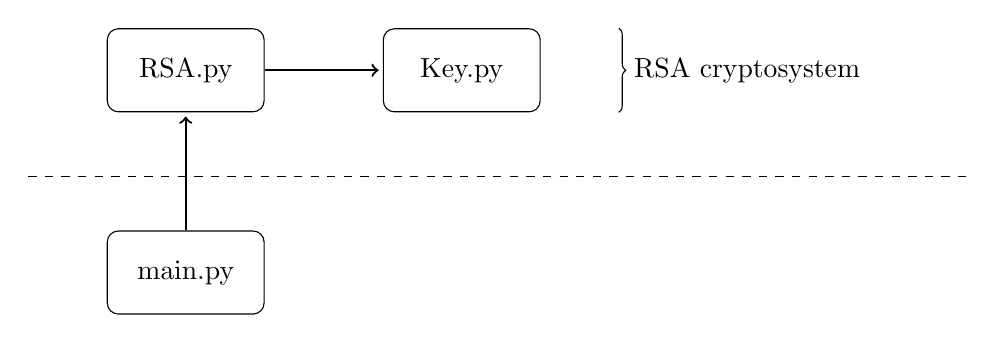
\begin{tikzpicture}
        [node distance=1.5cm]

        \node[block] (rsa) {RSA.py};
        \node[block,right=of rsa] (key) {Key.py};
        \node[block, below=of rsa] (main) {main.py};

        \draw[line] (rsa) -- (key);
        \draw[line] (main) -- (rsa);

        \draw[dashed] (-2, -1.35) -- (10, -1.35);

        \draw[tuborg, decoration={brace}] let \p1=(key.north), \p2=(key.south) in
            ($(5.5, \y1)$) -- ($(5.5, \y2)$) node[tubnode] {RSA cryptosystem};

    \end{tikzpicture}

    % Caption and Label
    \caption{System architecture}
    \label{fig:system}
\end{figure}

The system is going to be built using a library pattern and in fact it will allow any program
to use its contents to encrypt / decrypt messages. Consider that RSA is a slow algorithm compared
to symmetric algorithms.

\section{Rivest–Shamir–Adleman and public key cryptography}

RSA (Rivest–Shamir–Adleman) is a cryptosystem that was one of the first public-key based system.
That means that RSA have a public key and a private key used to share information between a sender
and a receiver.

\begin{figure}[H]
    \centering
    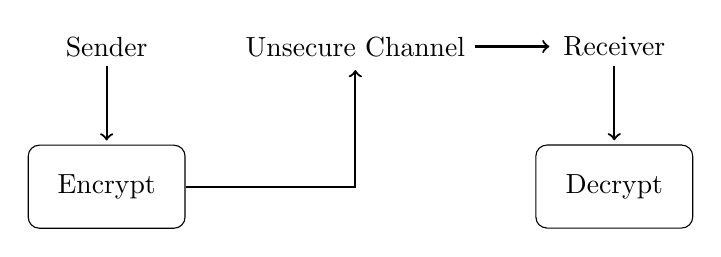
\begin{tikzpicture}
        [node distance=1cm]

        \node (sender) {Sender};
        \node[block, below=of sender] (encrypt) {Encrypt};
        \node[right=of sender] (channel) {Unsecure Channel};
        \node[right=of channel] (receiver) {Receiver};
        \node[block, below=of receiver] (decrypt) {Decrypt};

        \draw[line] (sender) -- (encrypt);
        \draw[line] (encrypt) -| (channel);
        \draw[line] (channel) -- (receiver);
        \draw[line] (receiver) -- (decrypt);

    \end{tikzpicture}

    % Caption and Label
    \caption{Transmission scheme}
    \label{fig:scheme}
\end{figure}

That said, the sender must first encrypt the message using the public key of the receiver.
Once the message is encrypted, it can be shared in a public channel that can be insecure by the pressence of
eavesdroppers. The message can only be decrypted by the receiver by using its private key. This can be achieved since
the public and the private keys share a mathematical relation. To further understand this concepts, the following explanation
corresponds to the RSA cryptosystem.

\subsection{Key Generation}

To generate a RSA key you need to follow the following steps:

\begin{itemize}
    \item Choose two prime numbers $p$ and $q$.
        Those numbers should be randomly chosen and should have a similar length in bits.
    \item Calculate $n = p \cdot q$. The result $n$ will be used as the modulus for both
        keys (private, public) and its length in bits designates the \textbf{key length}.
    \item Calculate $\Phi(n) = (p - 1) \cdot (q - 1)$. Euler's properties are used to calculate $\Phi$.
    \item Choose an $e$ that satisfies $e < \Phi$ and by having $e$ to be coprime with $\Phi$.
    \item Calculate $d$ given $e \cdot d \equiv 1 \mod \Phi$ (Modular multiplicative inverse)
\end{itemize}

The public key will be: \texttt{(n, e)} and the private key will be \texttt{(n, d)}

\subsection{Encryption}

The sender should share their public key in the public channel (it does not matter if anyone knows it).
The receiver would only need to share its public key in case of digital signature.
To demostrate an ecryption by using RSA let's consider the public key of the receiver as: \texttt{(n, e)} and its
private key \texttt{(n, d)}. The algorithm of \textit{Fast Modular Exponentiation} is used to calculate this operation.

If a sender wants to send the receiver a message it needs to encrypt the message by using the following mathematical formula:

\begin{center}
    $c \equiv m^e \mod n$
\end{center}

Consider $c$ to be the cipher text generated by the encryption.

\subsection{Decryption}

To decrypt, the same formula applies, but this time changing the $e$ with $d$.
Consider $c$ to be the cipher text generated by the encryption and this time, by using
$d$ (the private key) we can recover the original message.

\begin{center}
    $m \equiv c^d \mod n$ \\~\\
    $m \equiv (m^e)^d \mod n$ \\~\\
    $m \equiv m^{e \cdot d} \mod n \quad \rightarrow \quad p \equiv m^1 \mod n$ \\~\\
    $\boxed{m \equiv m \mod n}$
\end{center}

The end result $m$ is the original message that was sent.

\chapter{Implementation}

This chapter will include the implementation details of how to implement the given RSA Cryptosystem
using \textbf{Python 3}. The implementation, as mentioned earlier, will be done as a library containing
two modules \texttt{Key.py} and \texttt{RSA.py}

\section{RSA Key}

The RSA Key module (\texttt{Key.py}) is the one responsible of the key creation for the RSA cryptosystem.\\

The Key class will be used inside the RSA class to determine the current used key. Keep in mind that
the Key is able to automatically execute the steps mentioned in the key generation process given
two integers $p$ and $q$. This is done in the constructor and further saved into the class attributes.\\

The class atributes and methods are defined below. The method names contains the attributes needed to work.
They also have an brief explanation of what they do.

\begin{center}
    \begin{tabular}{ | l | p{6cm} |}
    \hline
    p, q, n, phi, e, d & The basic storage attributes for the RSA key as defined in the introduction.\\ \hline
    \_\_init\_\_(self, p = None, q = None) & Basic constructor to generate a key given $p$ and $q$. None values generate a prime from [50, 200]\\ \hline
    \_\_generate\_e\_and\_d(self) & Method to generate an e and d given $\Phi$ and $e$.\\ \hline
    \_\_generate\_e(self, phi) & Generate an $e$ based on $\Phi$.\\ \hline
    \_\_extended\_euclidean\_algorithm(self, a, b) & The Extended Euclidean Algorithm given $a = e$ and $b = \Phi$ to compute $d$ considering $d \cdot e \equiv \mod \Phi$.\\ \hline
    length(self) & Returnns the length of the key.\\ \hline
    public(self) & Returns the public key.\\ \hline
    private(self) & Returns the private key.\\ \hline
    print(self) & Prints the whole key (Public + Private).\\
    \hline
    \end{tabular}
\end{center}

\inputminted[linenos, breaklines=true]{python}{../Python/RSACryptosystem/Key.py}

\section{RSA Cryptosystem}

The RSA Class module (\texttt{RSA.py}) is the one responsible of the RSA cryptosystem.\\

The RSA class will be responsible of generating keys, encrypting and decrypting messages.
The key generation will be dispatched to the Key class, responsible of this things. The
RSA will only store and use the key.

The class atributes and methods are defined below. The method names contains the attributes needed to work.
They also have an brief explanation of what they do.

\begin{center}
    \begin{tabular}{ | l | p{6cm} |}
    \hline
    key & Stores the RSA key class used to encrypt / decrypt messages.\\ \hline
    \_\_fast\_modular\_exponentiation(self, a, z, n) & Method to calculate $x \equiv a^z \mod n$.\\ \hline
    generate\_key(self, p = None, q = None) & Method to generate a key given $p$ and $q$. If no value is provided, they are generated by Key class\\ \hline
    encrypt(self, plain\_text, e = None, n = None) & Encrypts a message (Might be a number or a string)\\ \hline
    decrypt(self, cipher\_text, d = None, n = None) & Decrypts an encrypted number or sequence of numbers (string).\\
    \hline
    \end{tabular}
\end{center}

\inputminted[linenos, breaklines=true]{python}{../Python/RSACryptosystem/RSA.py}

\chapter{Library Usage}

To use the library you simply need to import it as a regular \texttt{Python 3} library and use the RSA class
to access the given public methods. That said, the following example may ilustrate a sample usage case.

\inputminted[linenos, breaklines=true]{python}{../Python/main.py}

\begin{figure}[H]
    \centering
    \includegraphics[width=15cm]{RSA1}
    \caption{Example library output}
\end{figure}

\chapter{Simulation}

This simulation exposes a real live simulation to play around with the library.

The following simulation creates a sockets server and clients can connect to chat around.
During chatting, special commands may be used to setup the RSA cryptosystem and encrypt
messages to a given destination. All the available commands are:

\begin{center}
    \begin{tabular}{ | l | p{6cm} |}
    \hline
    K: $e$ $n$ & Send the public key to the public channel and others register it (should not be used).\\ \hline
    K: A & Sends the already generated key to the public channel (should be used).\\ \hline
    E: $x$ $m$ & Encrypts $m$ with the given saved public key $x$. $x$ is printed to the screen when the public key is registed.\\ \hline
    $m$ & Sends an insecure message $m$ to the public channel.\\
    \hline
    \end{tabular}
\end{center}

The following script is the chat server. It's reponsible of handling all the requests. It recieves all the
commands and sends them to all users in the channel. It's basically a broadcaster.

\inputminted[linenos, breaklines=true]{python}{../Python/chat_server.py}

In the other side, the following script corresponds to the chat client, where you connect
to the server and it's available to send all the listed commands.

\inputminted[linenos, breaklines=true]{python}{../Python/chat.py}

\begin{figure}[H]
    \centering
    \includegraphics[width=15cm]{RSA2}
    \caption{Socket server}
\end{figure}

\begin{figure}[H]
    \centering
    \includegraphics[width=15cm]{RSA3}
    \caption{Socket client 1}
\end{figure}

\begin{figure}[H]
    \centering
    \includegraphics[width=15cm]{RSA4}
    \caption{Socket client 2}
\end{figure}

\begin{figure}[H]
    \centering
    \includegraphics[width=15cm]{RSA5}
    \caption{Socket client 3}
\end{figure}

\chapter{Conclusions}

RSA Cryptosystems require more that what's explained here to be secure. As you may guess, the
same character is encrypted with the same ciphertext every time, leading to a deterministic cryptosystem.
However, by using \textbf{Optimal asymmetric encryption padding} you can avoid this problem. Deterministic systems
are subject to frequency analysis that may crack the system much faster.

The Key length must be quite large for the system to be secure nowadays, leading to a very big $n$ in bit length.
Nowadays standards go around key sizes of \textbf{2048 bits}.

\chapter{References}

Khan Academy. (2019). \textit{Fast modular exponentiation}.
[online] Available at:
\url{https://www.khanacademy.org/computing/computer-science/cryptography/modarithmetic/a/fast-modular-exponentiation}
[Accessed 12 Jan. 2019].\\

Loyola University Chicago. (2019). \textit{Extended Euclidean Algorithm}. 1st ed.
[ebook] Boston, Massachusetts: Dr. Andrew Harrington, p.2. Available at:
\url{https://anh.cs.luc.edu/331/notes/xgcd.pdf}
[Accessed 12 Jan. 2019].\\

Wikipedia. (2019). \textit{RSA (cryptosystem)}.
[online] Available at:
\url{https://en.wikipedia.org/wiki/RSA_(cryptosystem)}
[Accessed 12 Jan. 2019].\\

Python. (2019). \textit{Python 3.7.2 Documentation}.
[online] Available at:
\url{https://docs.python.org/3/}
[Accessed 12 Jan. 2019].

\end{document}
